\begin{tikzpicture}
  \node[anchor=south west, inner sep=0] (img) {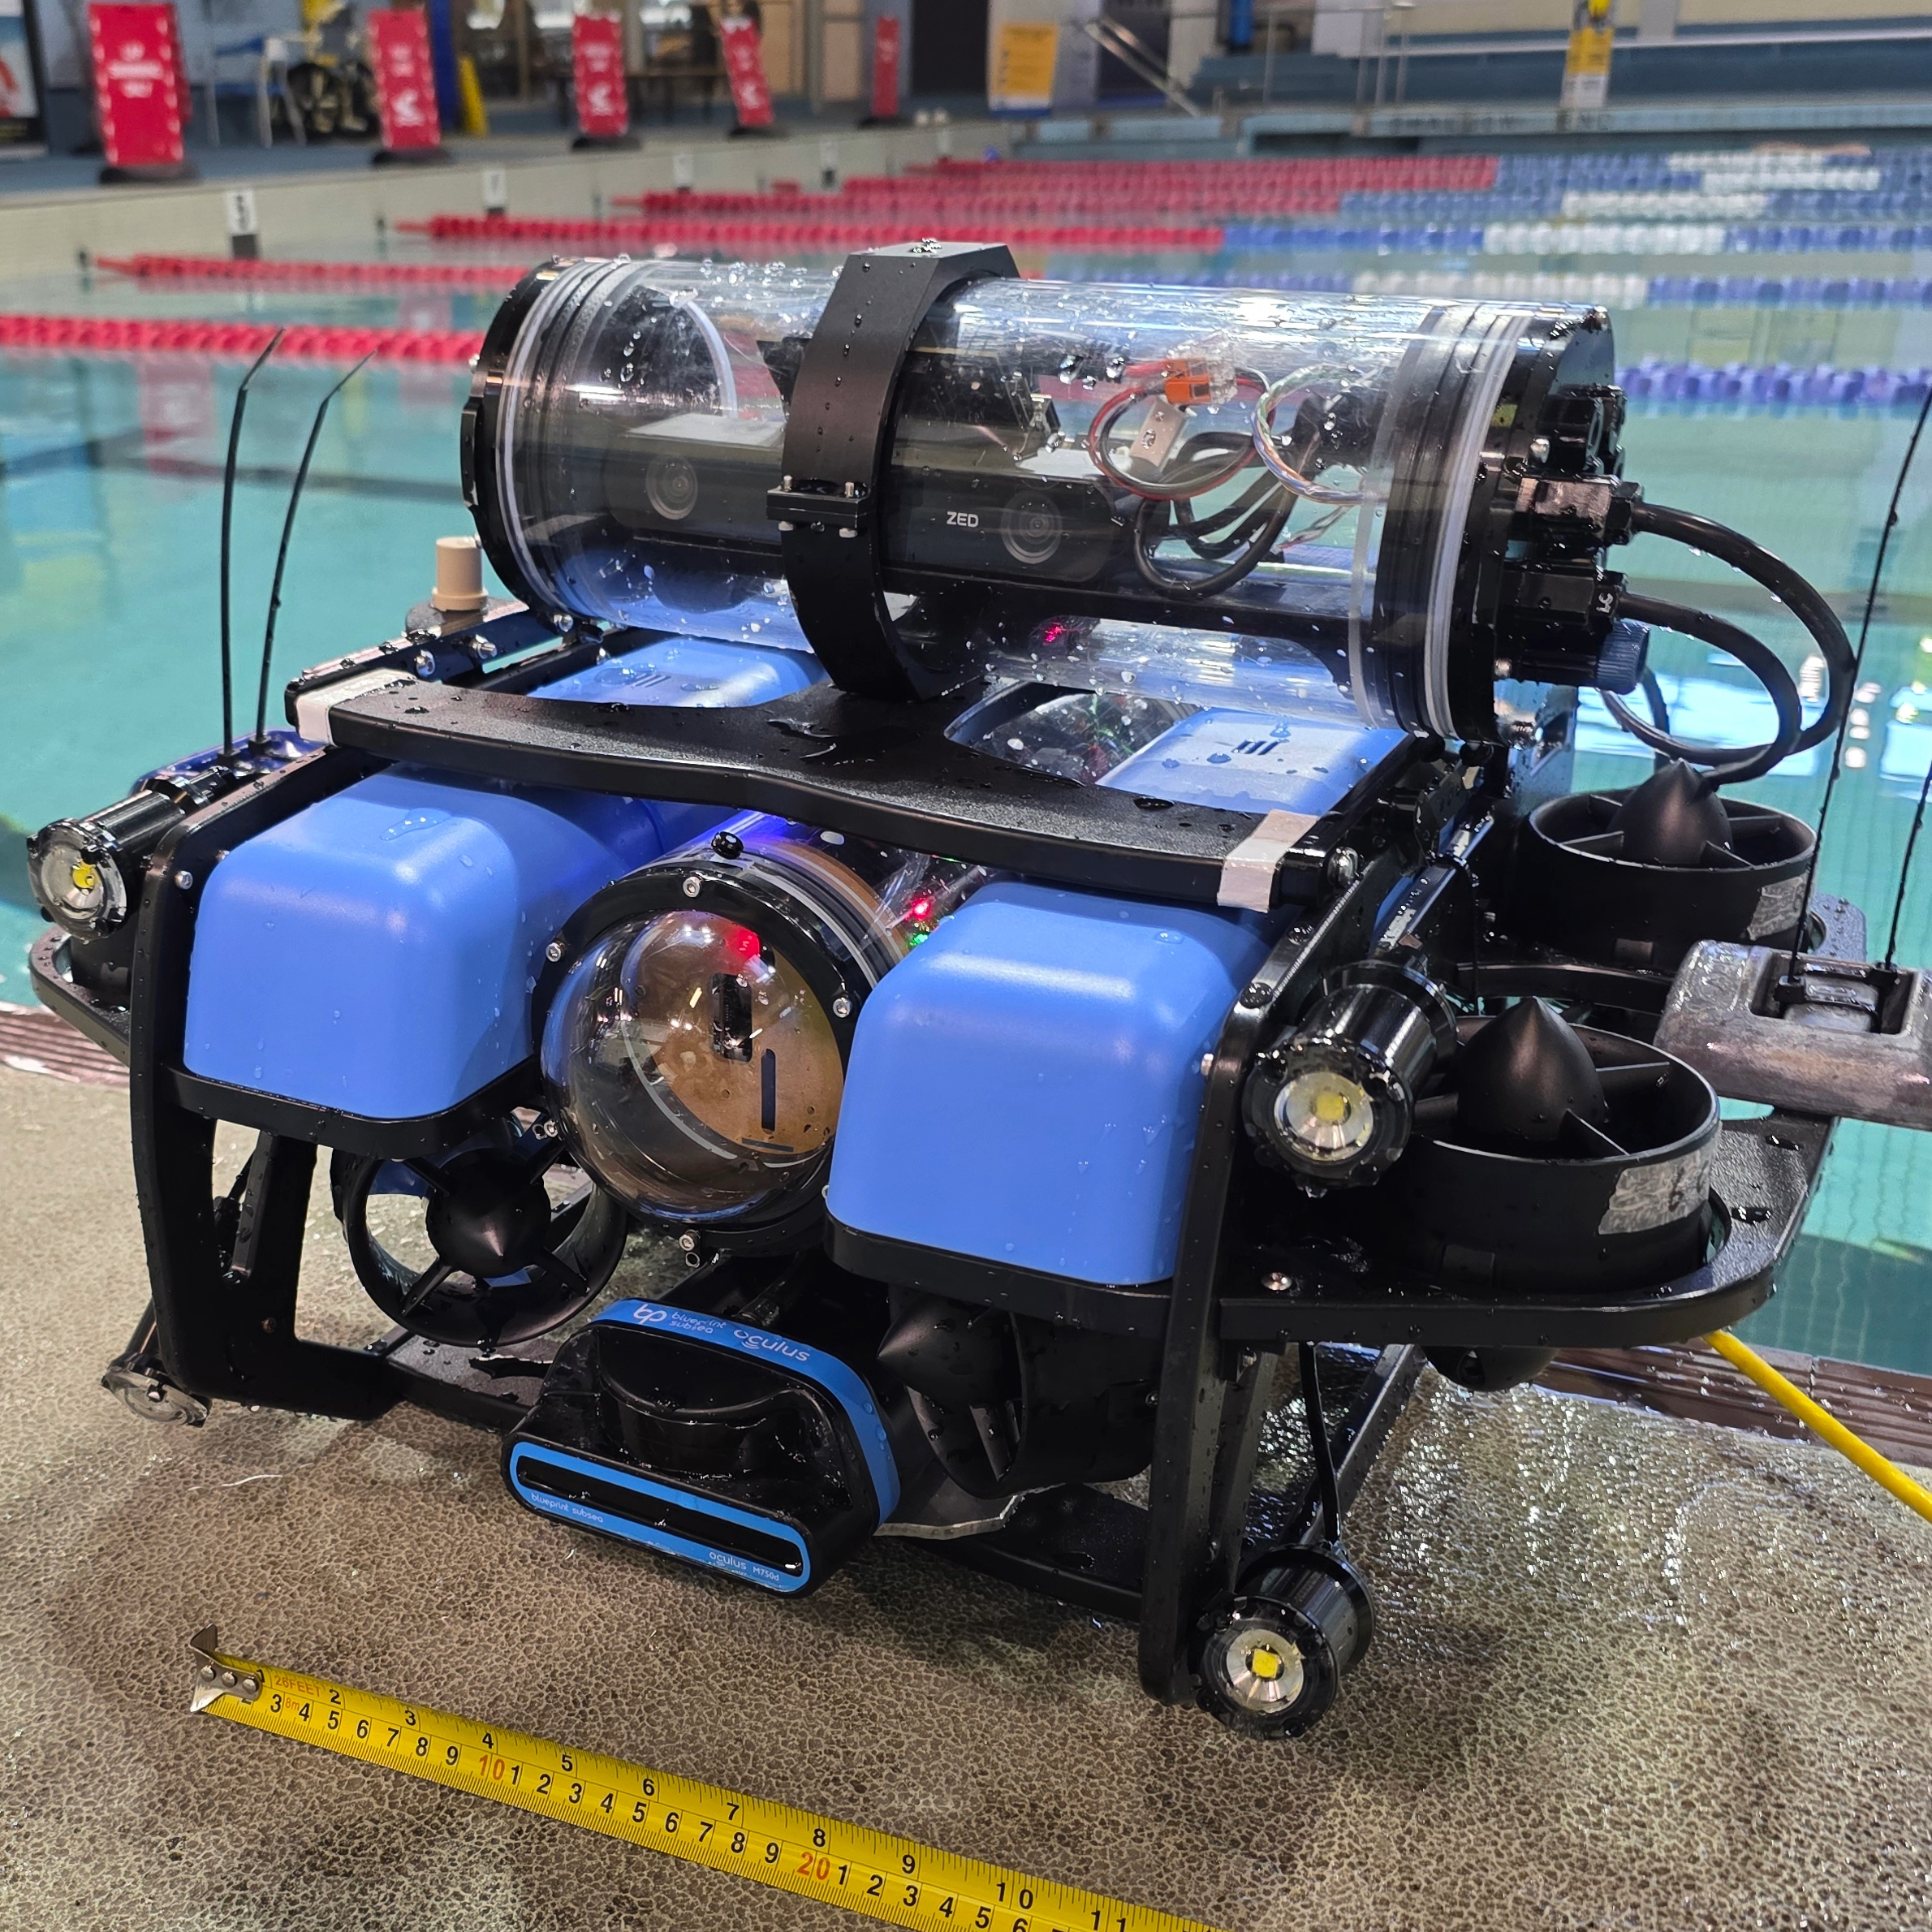
\includegraphics[width=0.45\textwidth]{Images/rov_zed_camera.png}};
  \begin{scope}[x={(img.south east)}, y={(img.north west)},
    lab/.style={font=\scriptsize\bfseries, text=white, align=center, fill=black, fill opacity=0.55,
        text opacity=1, inner sep=3pt, rounded corners=1pt},
    arr/.style={orange, thick, -{Stealth[length=1.6mm]}}]
    \node[lab] (lzed) at (0.20,0.93) {ZED stereo camera\\inside vacuum-sealed cylinder};
    \draw[arr] (lzed.south) to[bend right=10] (0.45,0.755);
  \end{scope}
\end{tikzpicture}
